%- in some cases search is still hard but the network operator might have an idea of what the path patterns might or might not look like - Done
%- example? - Done
%- a good way to express this is to add extra constraints of the form ... - Done
%- we formally define a subset of regexes that...?
%- algorithm
%- brief comparison with netgen
\section{Tactics} \label{sec:tactic}
If we consider reachability between two end-switches, the synthesis problem translates to choosing a path from the solution space of all paths from the source to destination such that the chosen path satisfies all policies like waypoints and isolation. Datacenter topologies have numerous paths between endpoints to provide full bisection bandwidth. This feature of datacenters ensues that the solution space of paths for a pair of endpoints is large. 

For example, consider the fat-tree topology in \cref{fig:fattree}. The number of paths under length 10 between two edge  switches in the same pod is 242 and two edge switches in different pods is 272. If we consider the synthesis of $n$ packet classes, the problem roughly translates to finding a solution in the solution space of size $n \times 242$ which satisfies all policies. 
\begin{figure}[H]
	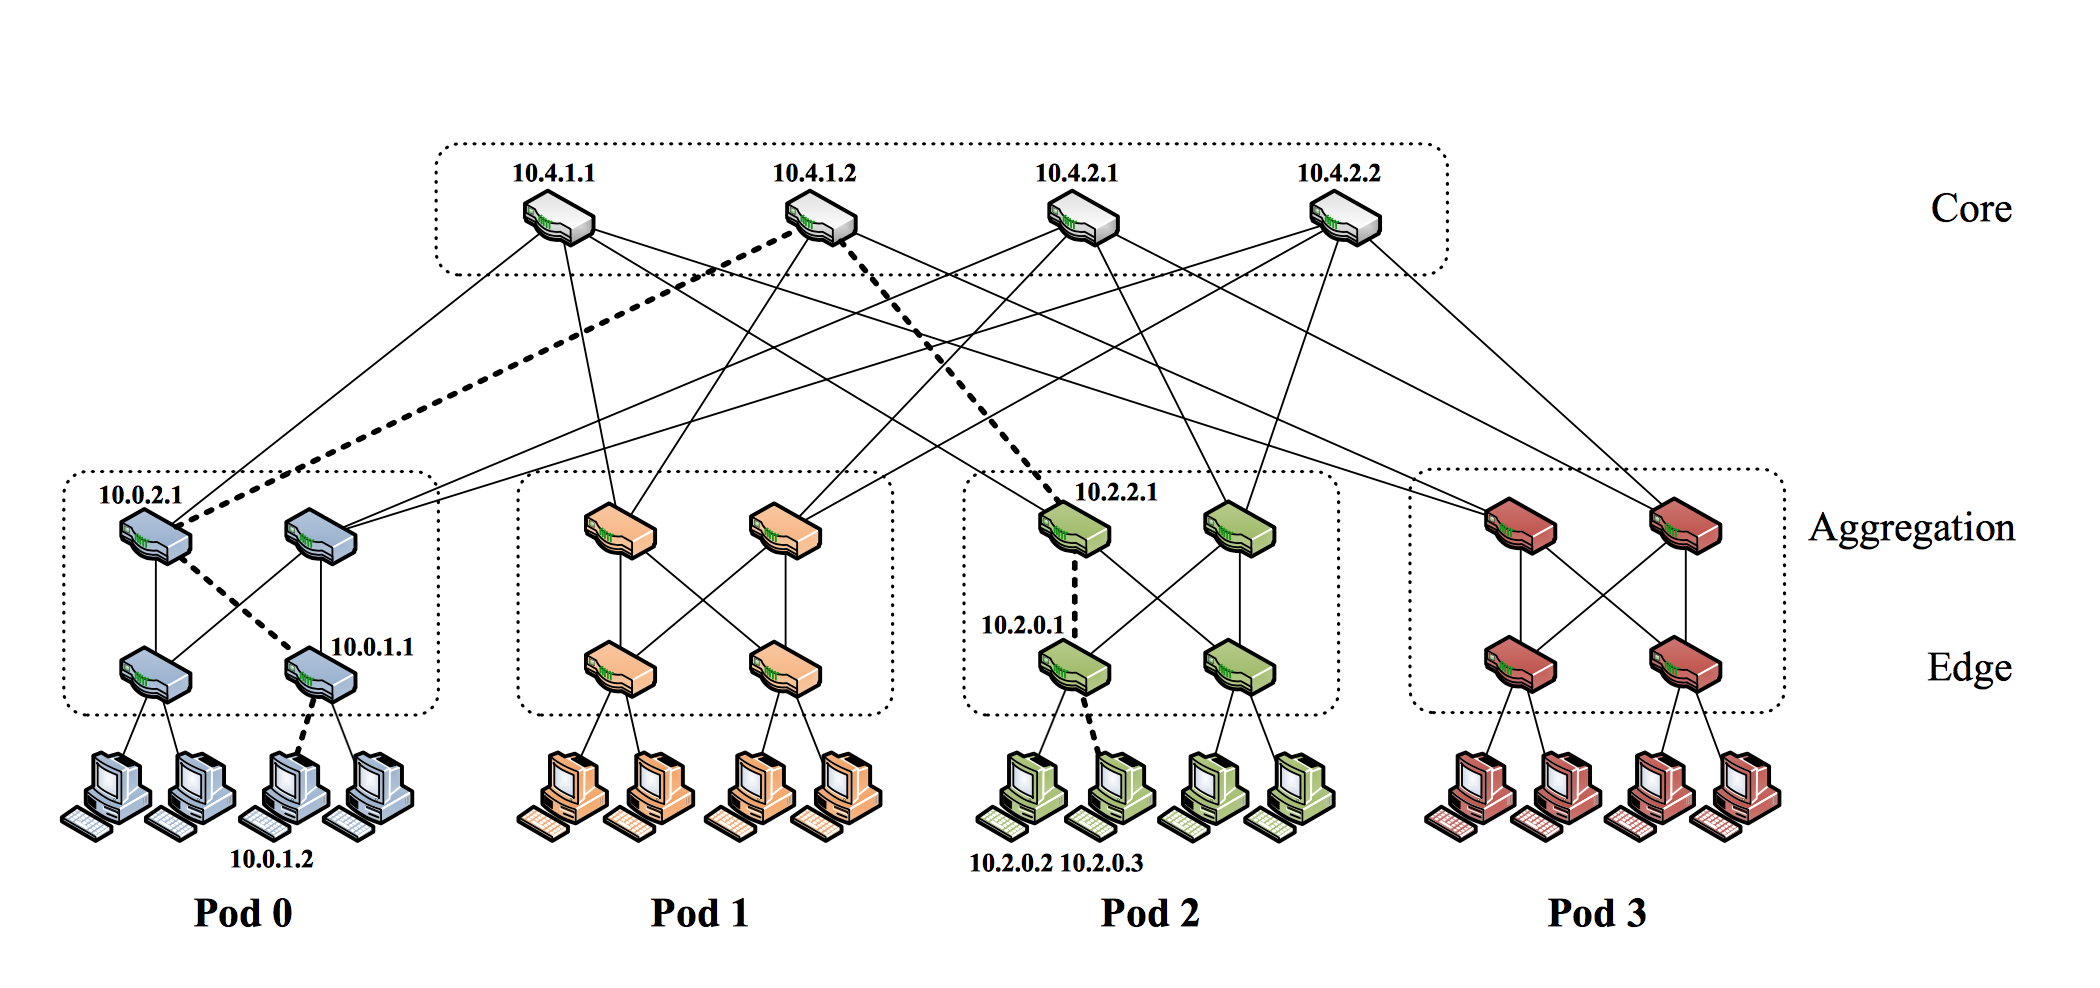
\includegraphics[width=\columnwidth]{fattree.png}
	\caption{Fat Tree Topology}
	\label{fig:fattree}
\end{figure}
Network operators can leverage the network structure of specific topologies to reduce the solution space by specifying patterns of what structure the path must or must adhere to. For example, In the case of \cref{fattree}, for a path from one edge to another, a reasonable pattern is that the path must not traverse another edge switch. This pattern will not drastically reduce the solution space of paths due to the dense interconnect between aggregate and core switches which can provide isolated paths for the different packet classes. 

Tactics and labels are abstractions that allow the operator to impose a high-level restriction on the paths by leveraging the network structure. We use the power of regular expressions and finite automata to prune constraints in our synthesis algorithm. To describe high-level restrictions on the path, we use the notion of mapping set of switches to labels to have a coarse grained control in describing the path. This ensures we do not reduce the solution space of paths drastically, and not being able to find a path satisfying all the policies.

 Let $Lb$ be the set of labels and $S$ be the set of switches in the topology. Let $\phi : S \rightarrow Lb$ be the labelling function that maps each switch to a label in $Lb$. One example for $\phi$ in the fat-tree topology in \cref{fig:fattree} can be that we map all switches in the same level (core, aggregate or edge) to the same label,
therefore leveraging the hierarchical structure of the topology. A path $p$ is a word over the alphabet $S$. Let $\Phi : S^* \rightarrow Lb^*$ be the path-labelling function which maps each switch in the word to its corresponding label. Let us consider a path $p = e1\ a2\ c3\ a4\ e2$. The label-path obtained by applying the path label function is $\Phi(p) = eacae$ (map each switch to its corresponding label).

\subsection{Synthesis with Tactics}
%We use regular expressions and finite automaton to prune the constraints and impose restrictions on the path. The natural way for operators to specify tactics are using \emph{blacklists}, which specify what the path should not be. To express this in a intuitive manner, we use regular expressions on the set of labels to specify blacklists. For example, to blacklist paths from a edge switch to edge switch to not go through another edge switch, we can describe the tactic as $\neg (e .^* e .^* e)$ where the label of all edge switches is $e$. Another tactic is of the form $\neg (e (.)^4 a c .* e)$ which specifies we have a path of length 4, we do not go in the direction towards the core (as to reach the edge, the path would have to then go downwards from the core). 
In NetGen \cite{netgen}, regular expressions are used to specify the path for the packet class.
While supporting full regular expressions is possible, it causes a blow-up in the solving time as further
constraints need to be added to the solver to ensure that path satisfies the regular expression, and operators would not be comfortable writing policy specifications in terms of regular expressions. Instead, using the notion of switch labels, we use regular expressions to provide high-level path properties as a search strategy rather than a policy requirement. Instead of specifying how the path must look like, we can use regular expressions on switch labels to specify \emph{blacklists}, how the path must not look like at a higher-level. A tactic, for example, is to blacklist paths from a edge switch to edge switch to not go through another edge switch. 
%\loris{we need a plot for the full regex thing to compare with Madhu, it would be great to repeat some of their experiments}
 
\subsubsection{Restricted tactic syntax}
We identified a restricted set of regular expressions that, not only do not require extra constraints to be added,
but actually allow us to avoid generating some of the constraints. 
This set is defined using the following grammar:
$$\begin{array}{rcl}
T  &  := & R | R \wedge T \\
R  &  :=  &  \neg (l_1 .^i C .^* l_2) \mid \neg (l_1 .^i l_2)\\ 
C  &  :=  &  \varepsilon \mid l_1 \mid l_1 l_2\\
\end{array}$$
where $l_i\in Lb$ and $l_1, l_2$ are used to specify the labels of the source switch and destination switch respectively of the packet classes. Thus, a tactic can be defined as the conjuction of regular expressions satisfying the restricted grammar $R$. 
Here, we allow some regular expressions to be negated at the outer level to specify blacklists. For example, $\neg (e .^i e .* e)$ says that the path must not contain a edge switch at the $i+1^{th}$ step, unless it is the destination switch. 
Similarly, $\neg (e .^i)$ says that...\loris{complete}
Let $\pi = sw_0\ldots sw_k$ be a path and 
let its labeling be $\phi(\pi)= a_0\ldots a_k$.
Se say that $\pi$ satisfies a tactic $R$, $\pi\vDash R$, if the following
holds:
\begin{itemize}
\item $\pi \vDash \neg R'$ iff $\pi \not\vDash R'$;
\item $\pi \vDash  l_1 .^i l_2$ iff $k\geq i+1$, $l_1= a_1$, and $l_2= a_k$; 
\item $\pi \vDash  l_1 .^i c.^* l_2$ iff $k\geq i+2$, $l_1= a_0$, $l_2= a_k$, and $a_{i+1}=c$;
\item $\pi \vDash  l_1 .^i c_1 c_2.^* l_2$ iff $k\geq i+3$, $l_1= a_0$, $l_2= a_k$, $a_{i+1}=c_1$, and $a_{i+2}=c_2$.
\end{itemize}

Notice that using this constraints we can express more complex forms such as
$\neg (e .* e .* e)$ which can be expressed in the restricted tactic syntax as $\bigwedge \limits_{i=0}^{i=\mu-2} \neg (e .^i e .^* e)$ where $\mu$ is the synthetic limit on path length.

\subsubsection{Tactic Synthesis Algorithm}
In our synthesis algorithm, the backward reachability propagation constraints (\cref{eq:bckprop}) ensure there is a path from source to destination. To incorporate tactics in the path, we need to modify these constraints. For a path $\pi = sw_0 \ldots sw_k$ and labelling $\Phi(\pi) = a_0 \ldots a_k$, we describe the modifications of the constraints for each type of tactic.

To satisfy tactics of the form $l_1  .^i c .^* l_2$ where $c \not= l_2$, the modifications are as follows :
\begin{multline} \label{eq:t1}
\pi \vDash \neg (l_1 .^i c .^* l_2) \wedge c \not= l_2 \Leftrightarrow \\ \forall sw. \phi(sw) = c \implies \neg Reach(sw, pc, i + 1)
\end{multline}
If $l_2 = c$, then \cref{eq:t1} will not work, as $l_1 .^i l_2$ satisfies the tactic, and thus for switches with label $c,Reach(sw,pc,i+1)$ can hold. The correct modifications are as follows which say that a switch with label $l_2$ cannot be succeeded by another switch (can only exist at the end of the path) : 
\begin{multline} \label{eq:t2}
 \pi \vDash \neg (l_1 .^i c .^* l_2) \wedge c = l_2 \Leftrightarrow \\ 
 \forall n_1. Reach(n_1,pc,i + 2) \implies \exists n_2.  n_2 \in N(n_1) \wedge \\ \phi(n_2) \not= c \wedge 
 Reach(n_2,pc,i+1) \wedge Fwd(n_2,n_1,pc)
\end{multline}
To satisfy tactics of the form $l_1  .^i c_1 c_2 .^* l_2$, the modifications are as follows to ensure that switch with label $c_2$ reached after $i + 2$ steps is not preceded by a switch of label $c_1$ : 
\begin{multline} \label{eq:t3}
\pi \vDash \neg (l_1 .^i c_1 c_2 .^* l_2) \Leftrightarrow \\ 
\forall n_1. \phi(n_1) = c_2 \wedge Reach(n_1,pc,i + 2) \implies \exists n_2.  n_2 \in N(n_1) \wedge \\ \phi(n_2) \not= c_1 \wedge 
Reach(n_2,pc,i+1) \wedge Fwd(n_2,n_1,pc)
\end{multline}
Incorporating tactics in the synthesis is sound and will always yield a correct path satisfying all policies but since tactics impose restrictions on the path, the synthesis algorithm is incomplete. However, tactics can be used to specify restrictions which would be reasonably complete, and speed up the synthesis, especially in datacenter topologies which are hierarchical and can be used to specify interesting tactics. 

\loris{For that restricted set of regexes the algorithm is trivial you should write the first pass. 
See the simplified syntax.
I'll help you with the proof but essentially you have to show that
if a path $sw_1\ldots sw_k$ satisfies the tactic regex then it is removed (i.e. all constraints necessary
for it to be encoded have been removed).
Other direction: if a path was in the original set of constraints and did not 
satisfy the tactic it has not been removed (also pretty easy)
}
\kausik{I think the tactics are quite intuitive to not need a proof of correctness. Do you think we need to explain how we came upon the restricted syntax?
}
\loris{No proof is fine. Some intuition would help. Give an example of one that locality can't handle.}

\subsection{Label Automaton}
Tactics are an intuitive way to express path properties leveraging the network structure using regular expressions. However, not every permutation of the label alphabet is a valid path in the topology, for example $eaae$ as the aggregate switches are only connected to edge or core switches. Under closer inspection, for a path from an edge switch to another edge switch, we can see that aggregate switches can only occur at odd path length. We describe a label automaton and the algorithm to prune constraints using switch label adjacencies. 

The label automaton $A^L$ is an automaton which accepts all words over the alphabet $Lb$ which are a labelling of a valid path in the topology in the topology and rejects all other words. The label automaton has state for each label and transitions for those labels which are connected to that label. We construct the label automaton for the fat-tree topology(\cref{fig:fattree}) in \cref{fig:labelauto}.  

\begin{figure}[h!]
	\centering
	\begin{tikzpicture}[shorten >=1pt,node distance=2cm,on grid,auto] 
	\node[state,initial] (q_0)   {$q_0$}; 
	\node[state,accepting] (q_a) [right=of q_0] {$q_a$}; 
	\node[state, accepting] (q_e) [above=of q_a] {$q_e$};
	\node[state,accepting] (q_c) [below=of q_a] {$q_c$}; 
	\path[->] 
	(q_0) edge  node {e} (q_e)
	edge node {a} (q_a)
	edge node {c} (q_c)
	(q_e) edge [bend right=30]  node {a} (q_a)
	(q_a) edge [bend right=30] node {e} (q_e)
	edge [bend right=30] node {c} (q_c)
	(q_c)[bend right=30] edge node {a} (q_a);
	\end{tikzpicture}
	\caption{Label automaton $A^L$ for fat-tree topology}
	\label{fig:labelauto}
\end{figure}
For a path starting from an edge switch,  
using a dynamic programming approach, we build sets $\Gamma(k)$ which is the set of all words starting with $e$ and of length $k$ accepted by the label automaton $A^L$ : $w \in \Gamma(k) \Leftrightarrow w \in L(A^L) \wedge |w| = k$. The algorithm computes $\Gamma(k-1)$, and then the last character of each word can be used to find the state the automaton is in(the automaton reaches the state after reading a particular label), and make a valid transition from that state to construct a word of size $k$ to compute  $\Gamma(k)$. 

Let us define $\Delta(k) := Lb \setminus \{l \ | w \in \Gamma(k) \wedge w[k] = l\}$ to the set of labels which cannot be reached by a path of length $k - 1$ (the length of the label word is one more than length of the path) from an edge switch. For example, in the fat-tree topology in \cref{fig:fattree}:
\[
\Delta(1) = \{c, e\} \ \ \ \Delta(2) = \{a\} \ \ \ \Delta(3) = \{c,e\}
\]
For each $k \leq \mu$, we can add the following constraints for packet classes which have traverse from a edge-to-edge switch to prune the backward reachability propagation constraints \cref{eq:bckprop}: 
\begin{equation}
	\forall sw. \phi(sw) \in \Delta(k) \implies (sw, pc, k -1) \notin Reach
\end{equation}
The label automaton pruning is sound and complete because we are using the network structure and labelling to prune certain constraints which cannot be valid. 
